\chapter{Generalidades}
    En este cap\'itulo se presenta de manera detallada los objetivos del proyecto, adem\'as de la informaci\'on de la instituci\'on donde ser\'a desarrollado el mismo.
    
    \section{Objetivos}
    En esta secci\'on se detallan los objetivos tanto generales como espec\'ificos a cumplir a lo largo del desarrollo del Sistema Integral de Indicadores.

\subsection{Objetivo general}

Desarrollar un sistema que permita medir, evaluar y controlar los procesos realizados por cada departamento en el Instituto Tecnol\'ogico de Tl\'ahuac, basado en los lineamientos establecidos por el TecNM en el Sistema de Gesti\'on de Calidad, para lograr realizar una gesti\'on eficaz y de calidad de los mismos.
Este sistema permitir\'a visualizar los resultados de los indicadores de tal manera que los procesos podr\'an ser monitoreados de una manera pr\'actica y accesible.


\subsection{Objetivos espec\'ificos}
\begin{itemize}
    \item An\'alisis de requerimientos.
    \item Toma de datos y entrevistas.
    \item Desarrollo del sistema.
    \item Implementaci\'on de sistema en ambiente de pruebas.
    \item Implemetaci\'on de sistema en ambiende de producci\'on.
\end{itemize}

\section{Justificaci\'on}
\paragraph{}%parrafo 1

Dicho proyecto est\'a basado en la necesidad de contar con una herramienta que permita la evaluaci\'on autom\'atica de los procesos pertenecientes en el Sistema de Gesti\'on de Calidad del Instituto Tecnol\'ogico de Tl\'ahuac, esto debido a que no se cuenta con ning\'un sistema para la realizaci\'on de dicha evaluaci\'on, ya que actualmente los procesos se realizan de manera manual, teniendo as\'i procesos extensos y complicados.
El Sistema Integral de Indicadores facilitar\'a el trabajo realizado, agilizara los tiempos requeridos y permitir\'a con esto brindar un mejor servicio a la comunidad del Instituto Tecnol\'ogico de Tl\'ahuac, adem\'as de que dichos indicadores influyen directamente para la toma de decisiones ya que muestran informaci\'on acerca del cumplimiento de los objetivos, logrando como beneficio el perfeccionamiento de los procesos de la instituci\'on.


\section{Caracterizaci\'on de la empresa en la que particip\'o}
En esta secci\'on se detalla la informaci\'on general de la instituci\'on, as\'i como el \'area para la cual se desarrolla el proyecto.

\subsection{Datos generales de la empresa}
\begin{itemize}
    \item \textbf{Empresa:} Instituto Tecnol\'ogico de Tl\'ahuac.
    \item \textbf{Direcci\'on:} Av. Estanislao Ram\'irez No.301 Colonia Ampliaci\'on Selene C.P. 13420 Tl\'ahuac D.F.
    %\vspace*{1in}
    \begin{figure}[htb]
        \centering
        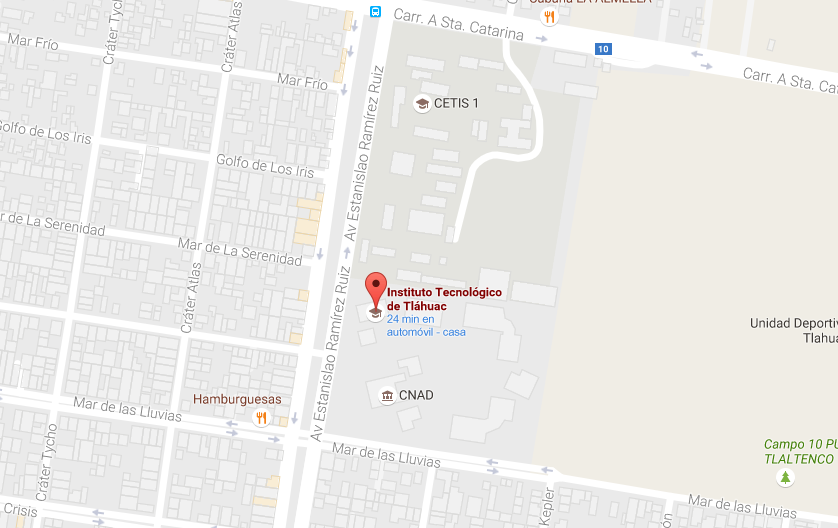
\includegraphics[width=14cm, height=9cm]{figuras/croquis}
        \caption{Croquis de ubicaci\'on.}
        \label{fig_croquis}
    \end{figure}
    \item \textbf{Tel\'efono:} 5866-0927, 7312-5616, 5841-0560, 2594-4096
    \item \textbf{Direcci\'on de correo electr\'onico:} sub.academica@ittlahuac.edu.mx
    \item \textbf{Giro:} 
    \item \textbf{Misi\'on:} Ofrecer un servicio educativo de calidad a trav\'es de la mejora continua, personal capacitado, compromiso global e infraestructura de vanguardia.

    \item \textbf{Visi\'on:} Ser una instituci\'on de alto desempe\~no acad\'emico, basada en la formaci\'on integral de profesionistas competitivos a nivel internacional con responsabilidad global.

    \item \textbf{Valores:}  Los valores que manejamos en la instituci\'on son los que nos ayudan a identificarnos como seres humanos, como personas que est\'an al servicio de la educaci\'on, que les gusta la actividad que desarrollan y que est\'an orgullosos de promover un servicio de calidad a la comunidad.
    \begin{itemize}
        \item Honestidad.
        \item Respeto.
        \item Trabajo en equipo.
        \item Vocaci\'on de servicio.
        \item Comunicaci\'on.
    \end{itemize}
    \item \textbf{Pol\'iticas de calidad:} La organizaci\'on establece el compromiso de implementar todos sus procesos orient\'andolos hacia la satisfacci\'on de sus estudiantes, sustentada en la calidad del proceso educativo, para cumplir con sus requisitos, mediante la eficacia de un sistema de gesti\'on de calidad de mejora continua, conforme a la norma ISO 9001:2008/NMX-CC-9001-IMNC-2008.
    
    \item \textbf{Estructura organizacional:} La estructura organizacional del Instituto Tecnol\'ogico de Tl\'ahuac se encentra como se muestra en la figura \ref{fig_organigrama}

    \begin{figure}[htb]
        \centering
        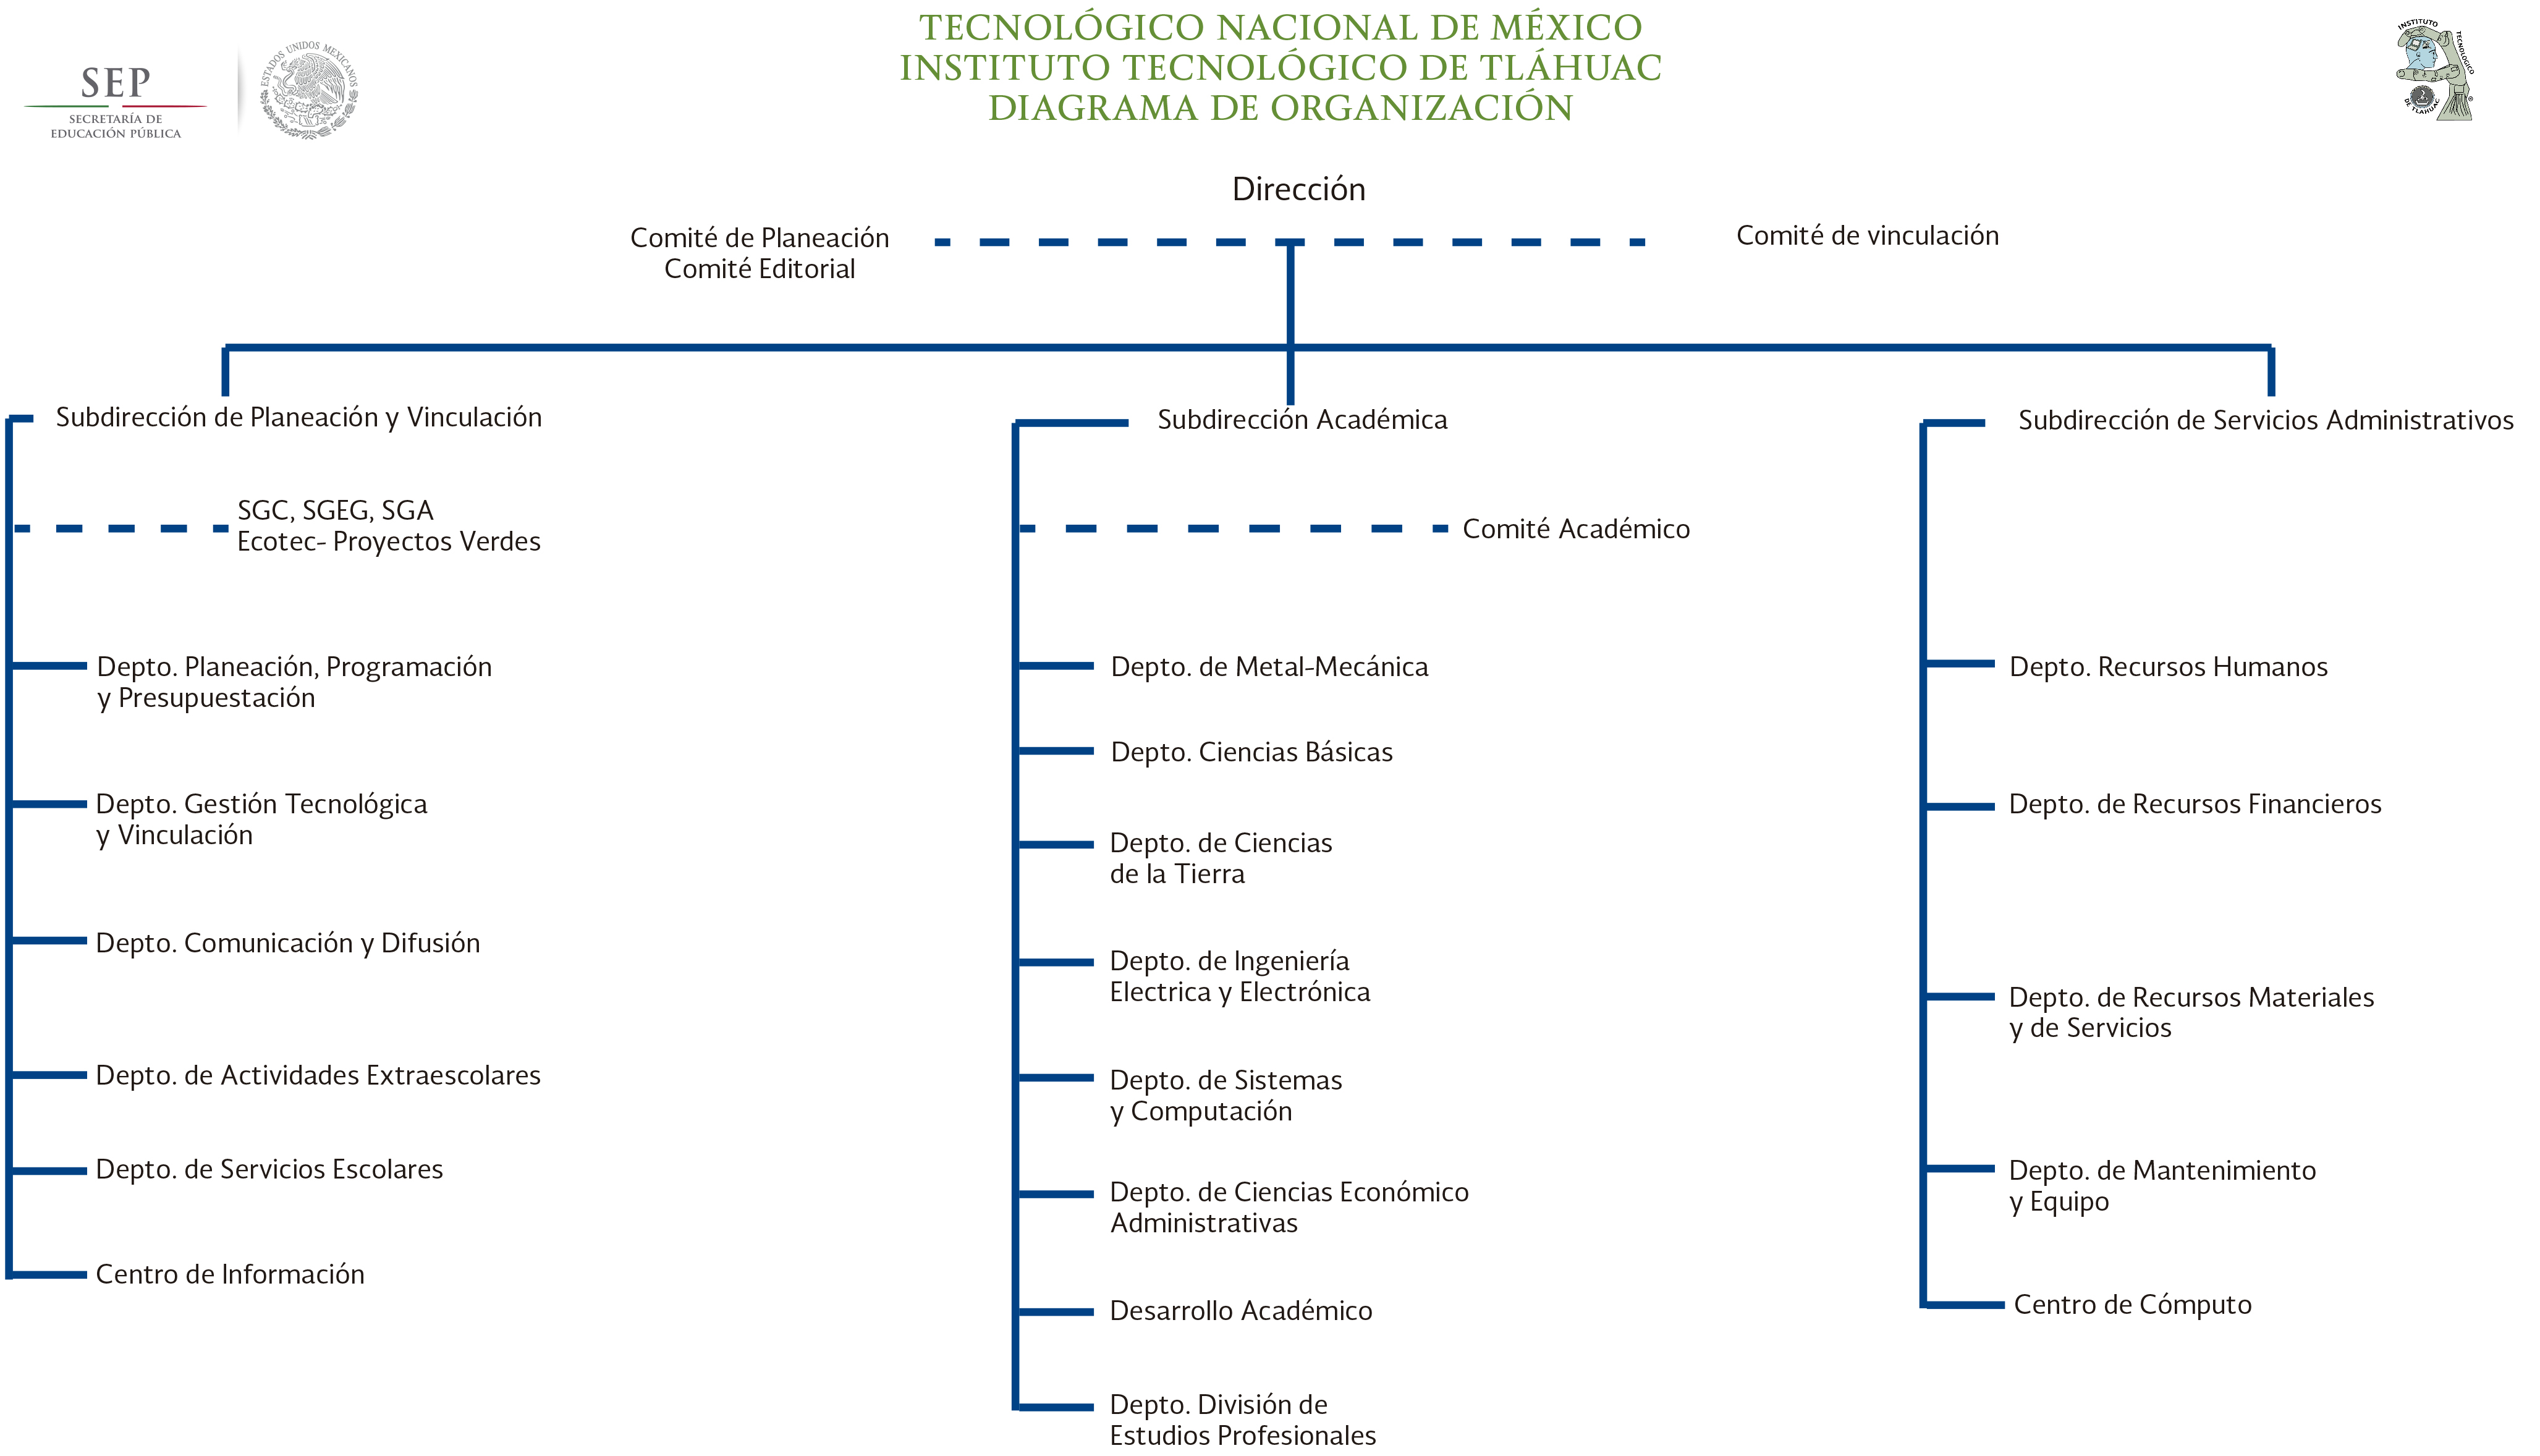
\includegraphics[width=14cm, height=9cm]{figuras/organigrama}
        \caption{Croquis de ubicaci\'on.}
        \label{fig_organigrama}
    \end{figure}
\end{itemize}

\subsection{Descripci\'on del departamento o \'area de trabajo.}
Definicion y detalle de el departamento.

\section{Problemas a resolver}
\paragraph{}%parrafo 1

A continuaci\'on se detallaran los problemas a resolver con el Sistema Integral de Indicadores.

Dentro de los problemas m\'as importantes a resolver se encuentra la digitalizaci\'on de los procesos de indicadores se realizan de manera manual. Esto por ende lleva demasiado tiempo y requiere de una gran sincronizaci\'on entre departamentos para que la informaci\'on sea confiable. Realizar estas actividades requiere de demasiado esfuerzo por parte de los trabajadores del Instituto Tecnol\'ogico de Tl\'ahuac lo que provoca que los tr\'amites sean lentos y tediosos. El Sistema Integral de Indicadores pretende solucionar este problema permitiendo tener la informaci\'on de los procesos en cualquier momento y de una manera sencilla, dando como resultado una sincronizaci\'on de informaci\'on eficiente y por consecuencia procesos m\'as r\'apidos.

Como segundo problema a resolver es la generaci\'on de datos indicadores para la toma de decisiones, la cual de igual manera que los procesos realizados en los departamentos, el sistema permitir\'a configurar reportes de indicadores para los directivos, permitiendo con esto tener informaci\'on general de los procesos.

Como \'ultimo punto el sistema contar\'a con la facilidad de adaptarse a nuevos procesos de indicadores, lo cual permite configurarse de tal manera que cuando la informaci\'on de un indicador cambie, esta modificaci\'on no necesite realizarse un cambio en c\'odigo.
